\documentclass[12pt]{article}
\usepackage{graphicx}
\graphicspath{{./images/}} % where to find images
\usepackage[labelfont=bf]{caption}

\begin{document}

\begin{figure}[!hbt]
  \centering
  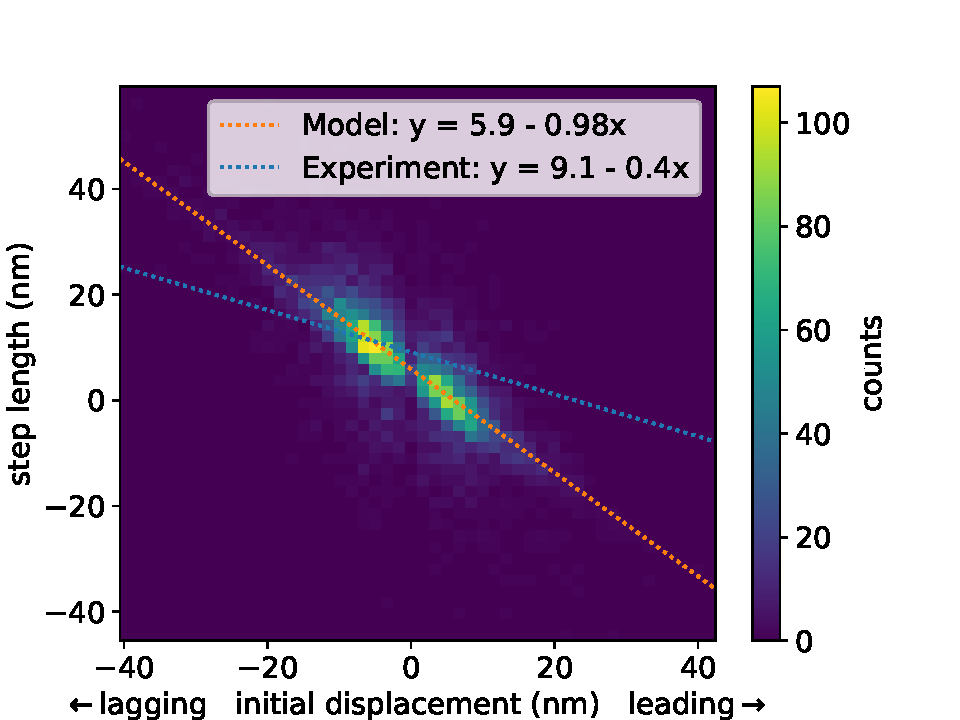
\includegraphics[width=0.75\columnwidth]{paper_displacement_vs_step_length}
  \caption{\textbf{Two dimensional histogram} comparing the total signed step length to
  the signed initial displacement between the binding domains. A positive value
  indicates that the front foot made the step (leading). A negative value
  indicates the rear foot (lagging) made the step. Simulations show a strong,
  negative correlation. A similar fit from an experimental paper is plotted for comparison.}
\end{figure}


\begin{figure}[!hbt]
  \centering
  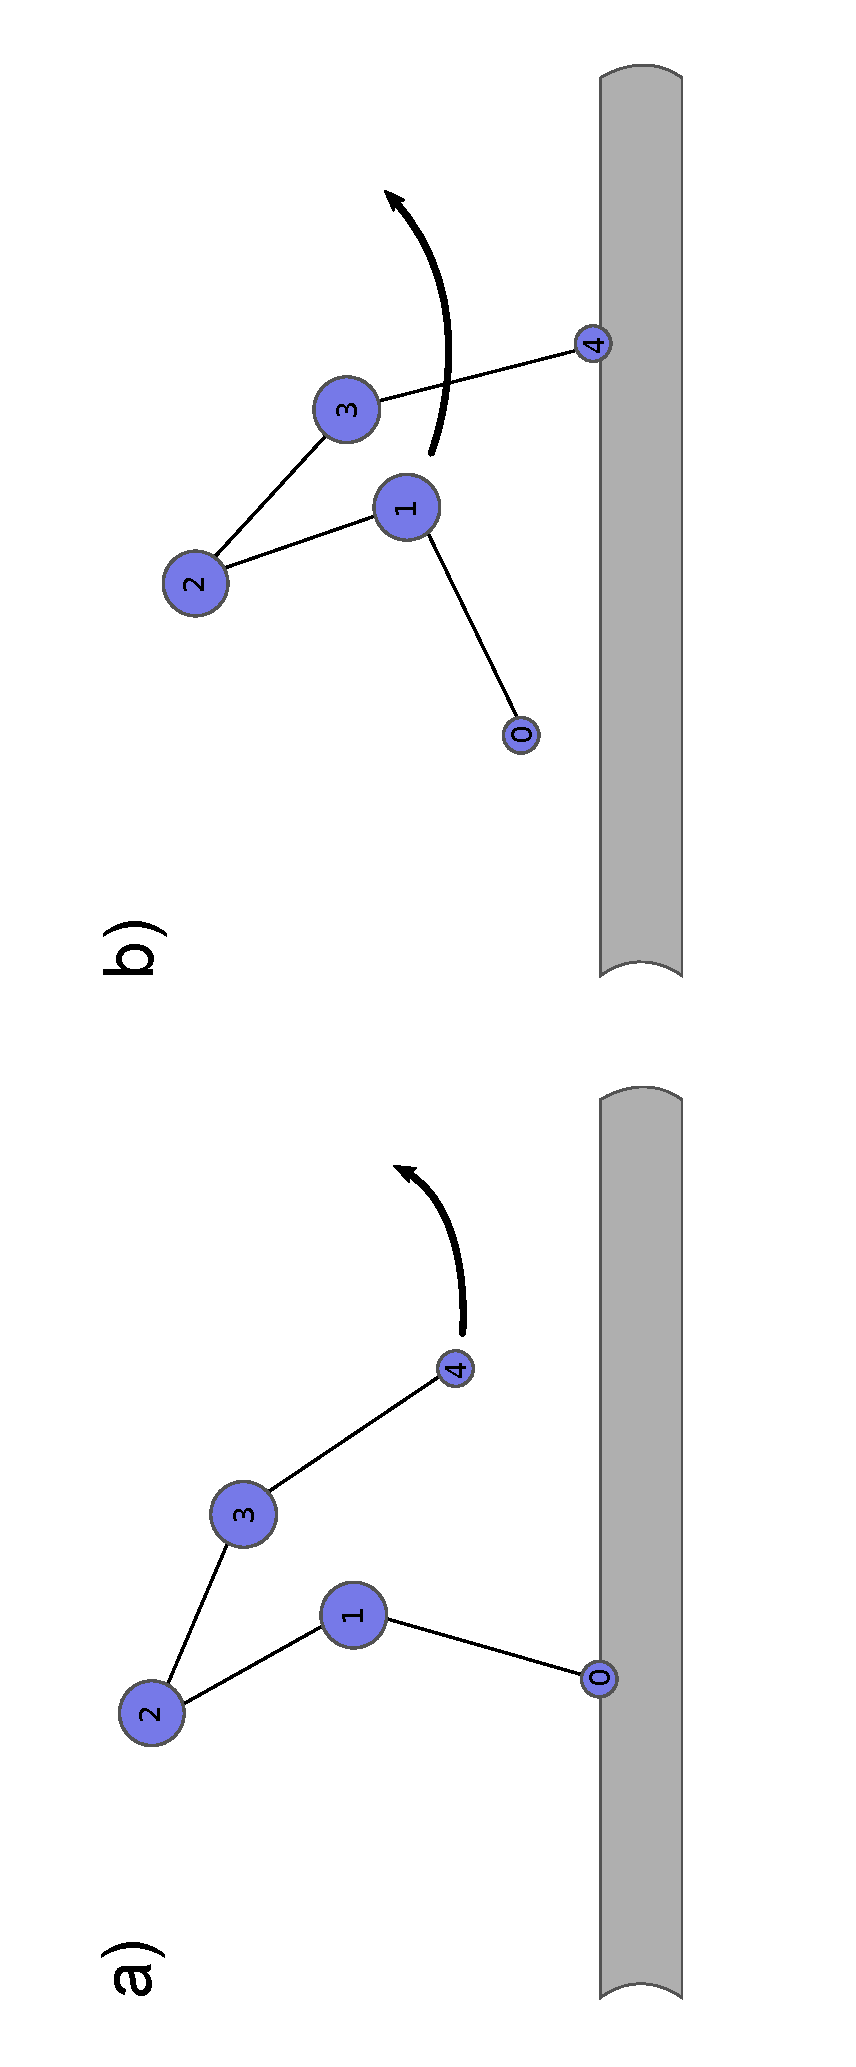
\includegraphics[angle=-90, width=1\columnwidth]{leading_vs_lagging}
  \caption{Diagram illustrating a leading foot step (a) and a lagging foot step (b).}
\end{figure}


\end{document}



